\begin{figure}[H]
	\centering
	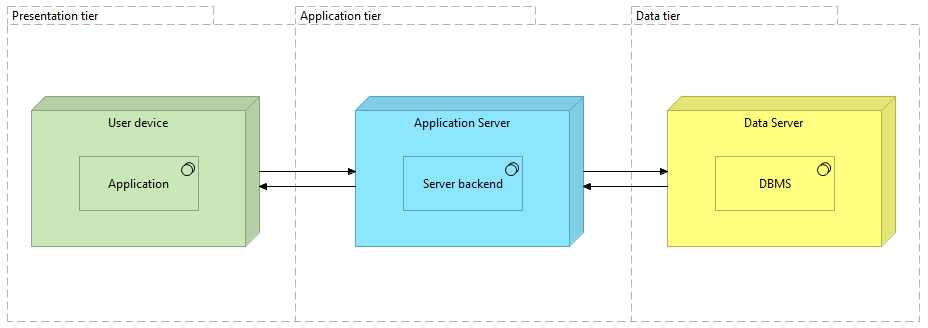
\includegraphics[width=\linewidth]{tier.png}
	\caption{Three-Tier architecture.}
\end{figure}

SafeStreets system is organized as a three-tier architecture, a standard design architecture used to provide a good level of security and performance thanks to subdivision of the tasks between the three tiers. Each tier runs on a different machine (or a group of machines with same structure), so that every tier is responsible of a specific task and the computational work is splitted between different machines, optimizing the performances of the overall system. This also improve the security of the system, because user devices need to pass through the application server to access the data and have no way to directly access it. 

The presentation tier runs directly on customers devices, which can be both smartphones running the official app or PCs using the web app, and its main goal is to handle the data and assets received by the application server to display the information on the device screen. User can then see the information requested and also interact with the presentation layer by using classical view widgets (like button, textfield, sliders, etc...) to require additional data based on their inputs. To summarize, the main goals of presentation layer are to allow communication with the application server API to require data based on user input and to visualize the results on the user's screen.

The application tier is composed by a replicated array of application servers, to scale horizontally the system using machines with the same structure and functionalities. The array of servers is managed by a load balancer, that distributes the clients' requests (and so the computational cost) equally between all the machines. Because application servers need to receive multiple requests from different clients in an efficient way, the load balancer integrates a router module that actively listens for any request made on specific server ports. The router has an handler for any endpoint of SafeStreets API that calls the manager related to the endpoint functionality, passing any input received in the request so that the manager can correctly consult or manipulate the database and produce an output, that is then returned by the router to the client that made that request. The list of managers that fulfil the functionalities is reported in a later section, in which every manager is also defined in detail.

The data tier's task is to provide access to data to the application tier, so that the manager modules can interrogate the database and also store or modify data in a reliable way. Data tier is composed by a single server, with cloned databases that share memory disks. This structure helps in maintaining high performances while keeping the data safe from possible hardware issues or data loss.

\begin{figure}[H]
	\centering
	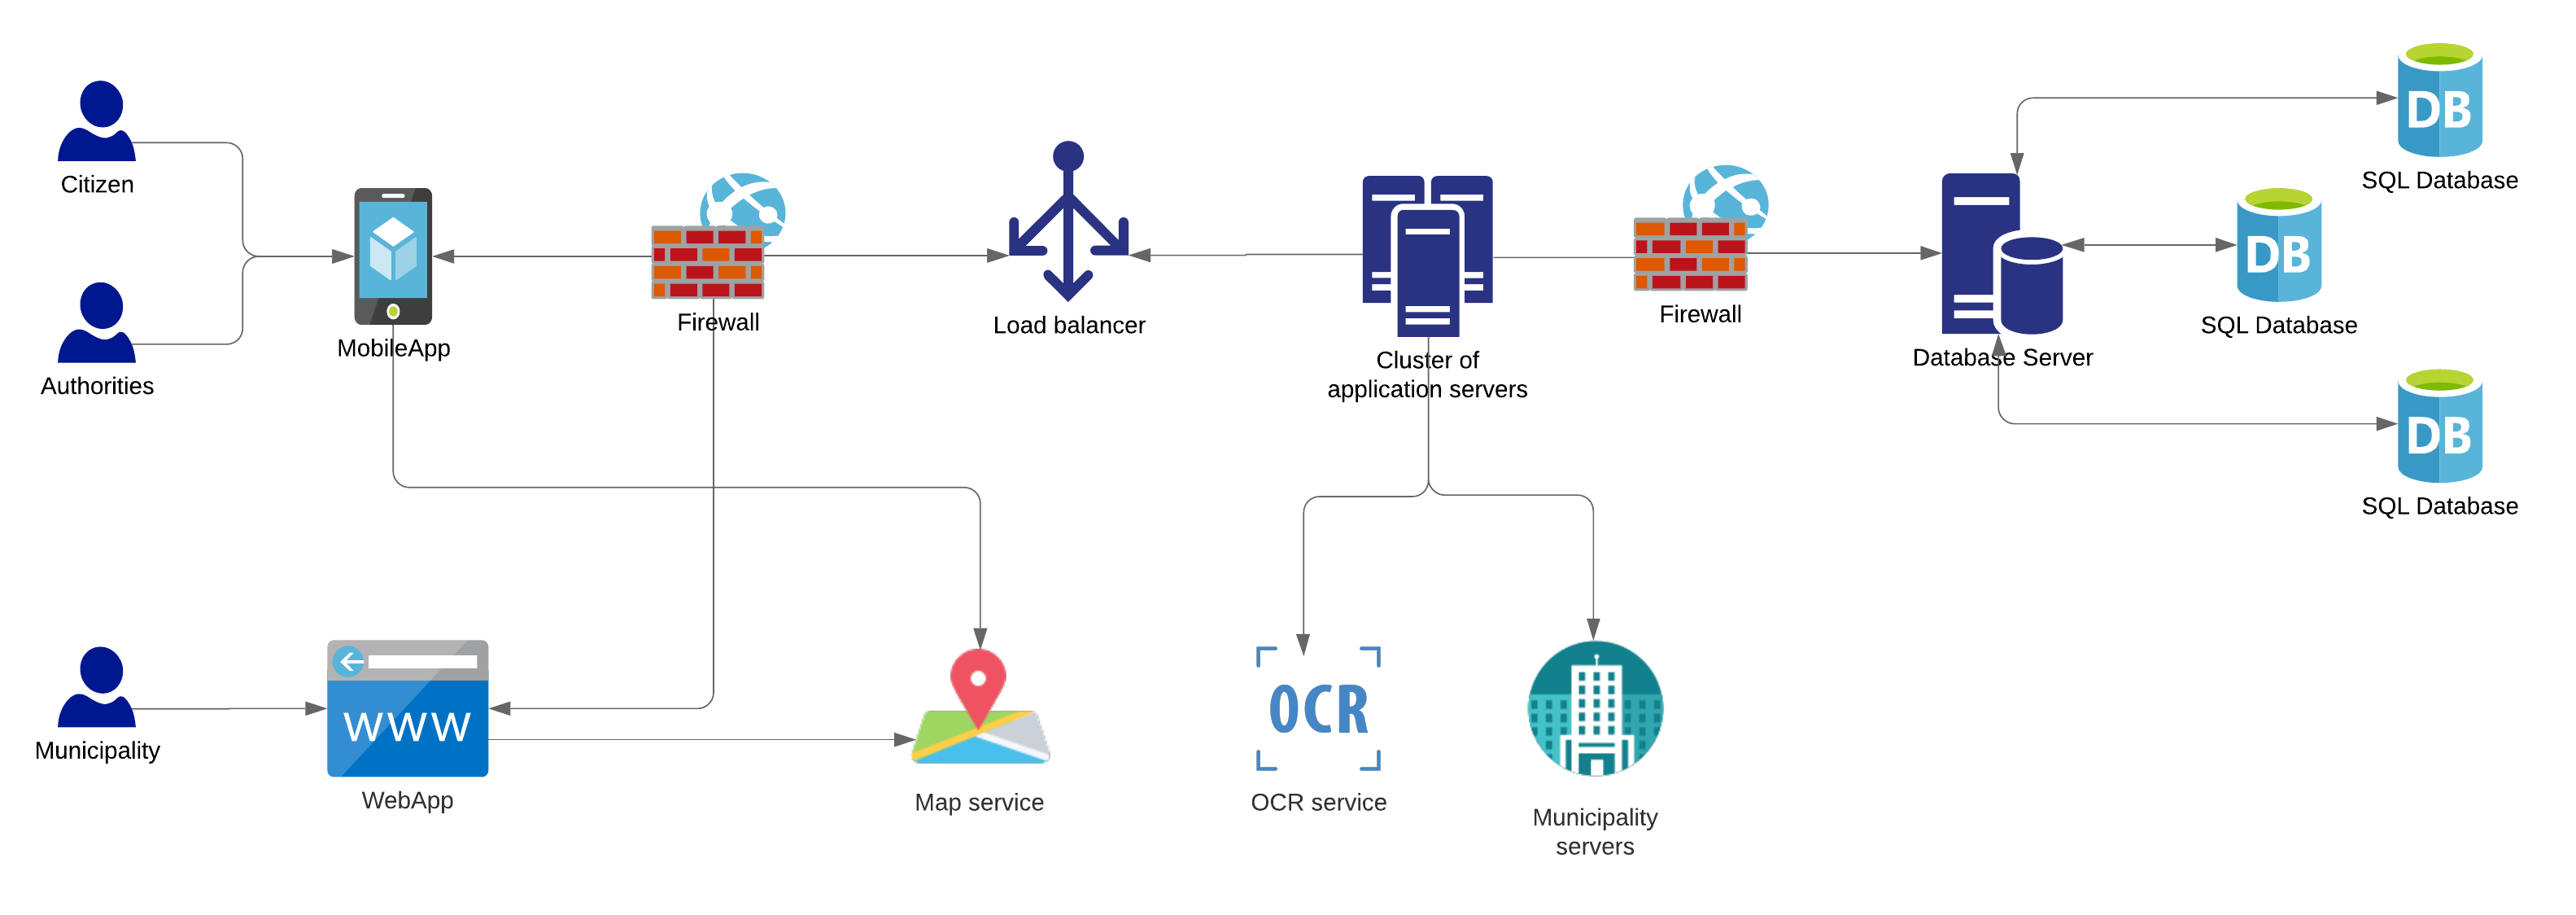
\includegraphics[width=\linewidth]{systemArchitecture.png}
	\caption{System architecture.}
\end{figure}

The three tiers are separated by firewalls to improve the security of the system. Firewall between application server and client is a must to provide a layer of protection from fraudulent users and hackers, because the application server could be accessed by anyone external to the system. The firewall between application server and database server isn't strictly necessary but can be used to negate all accesses that don't originate from the cluster of application servers, providing an additional layer of protection from fraudulent accesses.

The above system architecture diagram also shows the services external to SafeStreets system. A map service will be interrogated by all clients that need data visualization on a map, and the application server can call the API of a generic OCR service to recognize license plates of vehicles involved in reports from their photos, call the map service for metadata completion when registering a report, and can interact also with municipalities' API to integrate their data before generating the interventions.